\documentclass{article}
\usepackage{graphicx}
\usepackage{amsmath,amsthm,amssymb}
\usepackage[font=small,labelfont=bf]{caption}
\usepackage{tikz}
\usepackage{pgfplots}
\pgfplotsset{compat=1.18}
\usetikzlibrary{calc, angles, quotes, shapes.geometric, decorations.pathreplacing}
\usepackage{tkz-euclide}
\usepackage[inline]{asymptote}
\usepackage{float}
\usepackage[margin=1in]{geometry}
\usepackage{gensymb}
\usepackage[normalem]{ulem}
\usepackage{hyperref}
\hypersetup{
    colorlinks=true,
    linkcolor=blue,
    filecolor=magenta,      
    urlcolor=cyan,
    pdftitle={Overleaf Example},
    pdfpagemode=FullScreen,
    }
\usepackage{fancyhdr}
\pagestyle{fancy}
\fancyhead[R]{Enoch Yu}
\pagenumbering{gobble}
\usepackage{enumitem}
\newtheorem{theorem}{Theorem}[section]
\newtheorem{lemma}[theorem]{Lemma}
\newtheorem*{lemma*}{Lemma}
\newtheorem{sublemma}{Lemma}[section]
\newtheorem{proposition}{Proposition}
\newtheorem{corollary}{Corollary}[theorem]
\newtheorem{example}{Example}[section]
\newtheorem*{example*}{Example}
\newtheorem{hypothesis}{Hypothesis}[section]
\newtheorem*{hypothesis*}{Hypothesis}
\newenvironment{solution}{\begin{trivlist}\item[]{\bf Solution}}{\qed \end{trivlist}}
\newcommand{\verteq}{\rotatebox{90}{$\;\;=\;\;$}}
\newcommand*\circled[1]{\tikz[baseline=(char.base)]{
            \node[shape=circle,draw,inner sep=1pt] (char) {#1};}}
\newcommand{\triangled}[1]{\tikz[baseline=(char.base)]{
            \node[shape=regular polygon, regular polygon sides=3, draw, inner sep=0.2pt] (char) {#1};}}

\title{Problem Set 26}
\author{Enoch Yu}
\date{June 2025}

\begin{document}

\section*{2019 AMC 12A Problem 19}
In $\triangle{ABC}$ with integer side lengths,
\[
\cos A = \frac{11}{16}, \qquad \cos B = \frac{7}{8}, \qquad \text{and} \qquad \cos C = -\frac{1}{4}.
\]
What is the least possible perimeter for $\triangle{ABC}$?
\\\\
\begin{solution}
\\\\
\textbf{Key Word} Law of Sines
\\\\
\textcolor{red}{\textbf{YOU SHOULD BE FLEXIBLE ENOUGH TO THINK OF $\sin$ WHEN YOU SEE $\cos$!!!!}}
\begin{align*}
    \cos A = \frac{11}{16} &\implies \sin A = \frac{3\sqrt{15}}{16} \\
    \cos B = \frac{7}{8} &\implies \sin B = \frac{\sqrt{15}}{8} \\
    \cos C = -\frac{1}{4} &\implies \sin C = \frac{\sqrt{15}}{4}
\end{align*}
\begin{center}
    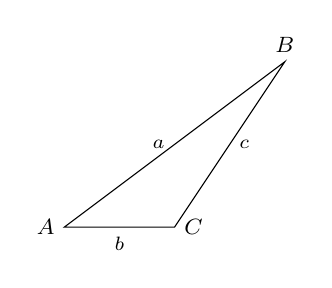
\begin{tikzpicture}[scale=0.7]
        \coordinate (A) at (0,0);
        \coordinate (B) at (4,3);
        \coordinate (C) at (2,0);

        \draw (A) -- (B) -- (C) -- cycle;

        \node[left] at (A) {\footnotesize $A$};
        \node[above] at (B) {\footnotesize $B$};
        \node[right] at (C) {\footnotesize $C$};

        \node[left] at ($(A)!0.5!(B)$) {\scriptsize $a$};
        \node[below] at ($(A)!0.5!(C)$) {\scriptsize $b$};
        \node[right] at ($(C)!0.5!(B)$) {\scriptsize $c$};
    \end{tikzpicture}
\end{center}
Therefore, using the law of sines, we could infer that the following expressions are true.
\begin{align*}
    \frac{a}{\sin A} = \frac{b}{\sin B} = \frac{c}{\sin C}
    &\Rightarrow \frac{a}{\frac{3\sqrt{15}}{16}} = \frac{b}{\frac{\sqrt{15}}{8}} = \frac{c}{\frac{\sqrt{15}}{4}} \\
    &\Rightarrow \frac{a}{3} = \frac{b}{2} = \frac{c}{4} \\
    \therefore &\Rightarrow a : b : c = 3 : 2 : 4
\end{align*}
Because $\triangle{ABC}$ has integer side lengths, $3 + 2 + 4 = \boxed{9}$.
\end{solution}

\newpage
\section*{2014 AMC 12B Problem 25}
Find the sum of all the positive solutions of
\[
2 \cos (2x) \left( \cos (2x) - \cos \left(\frac{2014 \pi^2}{x} \right) \right) = \cos (4x) - 1
\]
\begin{solution}
\\\\
\textbf{Key Word} Trigonometric Identities
\\\\
First and foremost, the equation above could be simplified using trigonometric identities.
\begin{align*}
    2 \cos (2x) \left( \cos (2x) - \cos \left(\frac{2014 \pi^2}{x} \right) \right) &= \cos (4x) - 1 \\[0.4em]
    2 \cos (2x) \left( \cos (2x) - \cos \left(\frac{2014 \pi^2}{x} \right) \right) &= (2\cos^2(2x) - 1) - 1 \\[0.4em]
    \cos (2x) \left( \cos (2x) - \cos \left(\frac{2014 \pi^2}{x} \right) \right) &= \cos^2(2x) - 1 \\[0.4em]
    \cos (2x) \cos \left(\frac{2014 \pi^2}{x} \right) &= 1
\end{align*}
Because $\cos$ functions are bounded by the interval $[-1,1]$, $\cos (2x) = 1$ and $\cos \left(\frac{2014 \pi^2}{x} \right) = 1$. In other words, $2x = 2n\pi$ and $\frac{2014 \pi^2}{x} = 2n'\pi$ where $\{ n, n' \} \in \mathbb{Z}$.
\begin{align*}
    2x &= 2n\pi \\
    x &= n\pi \\
    \frac{2014 \pi^2}{x} &= 2n'\pi \\
    \frac{1007 \pi}{x} &= n' \\
    \therefore x &= \frac{1007 \pi}{n'}
    \\\\
    x
    &\Rightarrow \pi, 19\pi, 53\pi, 1007\pi \\
    &\Rightarrow \pi + 19\pi + 53\pi + 1007\pi = \boxed{1080\pi}
\end{align*}

\end{solution}

\end{document}
